Let
\begin{align}
    \vec{n_1} &= \myvec{4 \\ 8} - \myvec{-2 \\ 6}\\
    &= \myvec{6 \\ 2}
\end{align}
and
\begin{align}
     \vec{n_2} &= \myvec{x \\ 24} - \myvec{8 \\ 12}\\
    &= \myvec{x - 8 \\ 12}
\end{align}
From the given information, 
\begin{align}
 \vec{n_1^\top}\vec{n_2}  &= 0\\
 \implies  \myvec{6 & 2} \myvec{x - 8 \\ 12}&=0
 \\
 \text{or, }    x = 4
\end{align}
Fig. \ref{fig:vec/2/36/1} verifies the result.
%
\begin{figure}[!ht]
    \centering 
    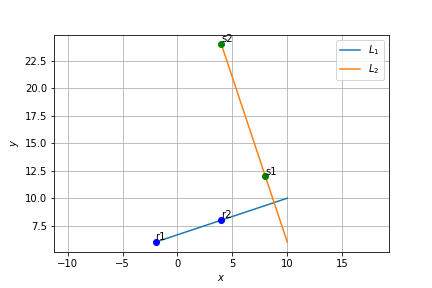
\includegraphics[width= \columnwidth]{solutions/su2021/2/36/assignment8.png}
    \caption{Lines $L_1$ and $L_2$}
    \label{fig:vec/2/36/1}
\end{figure}



